\documentclass[main.tex]{subfiles}
\begin{document}
\begin{bmcsex}{Bond damage}{e21_bond_slip_damage}
\noindent Single material point of a bond section is
    loaded monotonically showing the bond deterioration
    governed by a prescribed damage function $\omega$.
     \\
\begin{center}
            
{\scriptsize 
\begin{longtable}{lrp{4cm}}\toprule
\textbf{\textsf{Model parameter}} 
& 
\textbf{\textsf{Symbol = Value [Unit]}} 
&
\textbf{\textsf{Description}}  \\\midrule \midrule
\texttt{n\_steps} & $n_\mathrm{s}$ = 1000 [-] & {\footnotesize None}  \\
            \texttt{material\_model} & option = damage [-] & {\footnotesize None}  \\
            \texttt{interaction\_type} & option = predefined [-] & {\footnotesize None}  \\
            \midrule
\multicolumn{3}{l}{\textbf{\textsf{LoadingScenario: loading\_scenario}}}\\

\texttt{loading\_scenario.number\_of\_cycles} & $n_\mathrm{cycles}$ = 1 [-] & {\footnotesize None}  \\
            \texttt{loading\_scenario.number\_of\_increments} & $n_{\mathrm{incr}}$ = 20 [-] & {\footnotesize None}  \\
            \texttt{loading\_scenario.loading\_type} & option = cyclic [-] & {\footnotesize None}  \\
            \texttt{loading\_scenario.maximum\_loading} & $\phi_{\max}$ = 0.005 [-] & {\footnotesize None}  \\
            \texttt{loading\_scenario.amplitude\_type} & option = constant [-] & {\footnotesize None}  \\
            \texttt{loading\_scenario.unloading\_ratio} & $\phi_{\mathrm{unload}}$ = 0.5 [-] & {\footnotesize None}  \\
            \texttt{loading\_scenario.loading\_range} & option = non-symmetric [-] & {\footnotesize None}  \\
            
\multicolumn{3}{r}{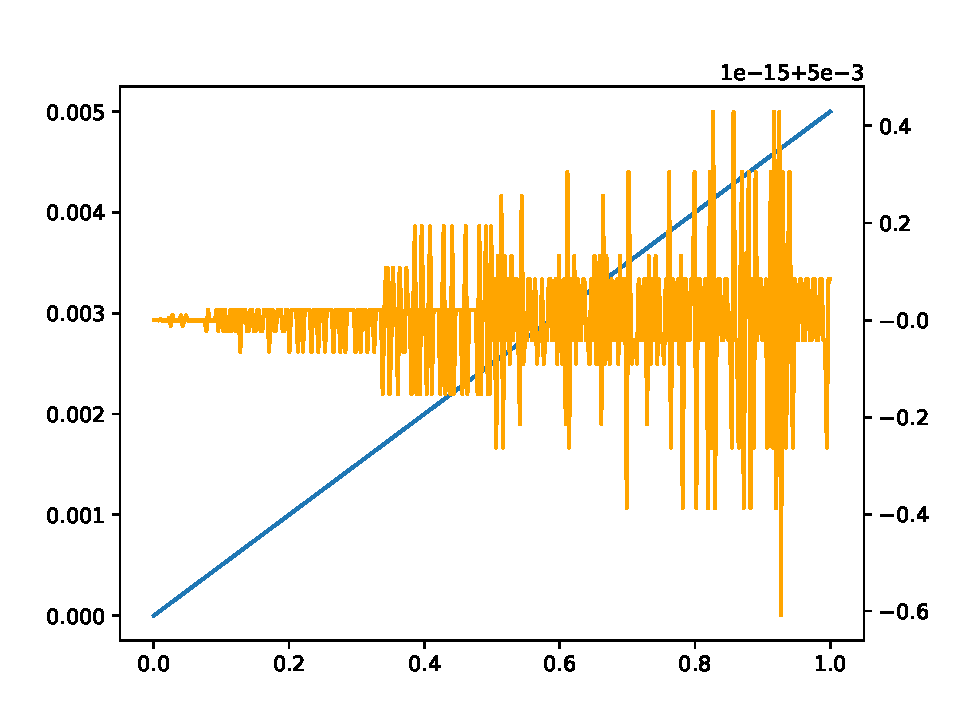
\includegraphics[width=5cm]{examples/e21_bond_slip_damage/fig_loading_scenario.pdf}}\\
\midrule
\multicolumn{3}{l}{\textbf{\textsf{MATSBondSlipD: mats\_eval}}}\\

\texttt{mats\_eval.omega\_fn\_type} & option = jirasek [-] & {\footnotesize None}  \\
            \midrule
\multicolumn{3}{l}{\textbf{\textsf{JirasekDamageFn: omega\_fn}}}\\

\texttt{mats\_eval.omega\_fn.s\_0} & $s_0$ = 0.0004 [None] & {\footnotesize elastic strain limit}  \\
            \texttt{mats\_eval.omega\_fn.s\_f} & $s_f$ = 0.003 [None] & {\footnotesize parameter controls the damage function}  \\
            
\multicolumn{3}{r}{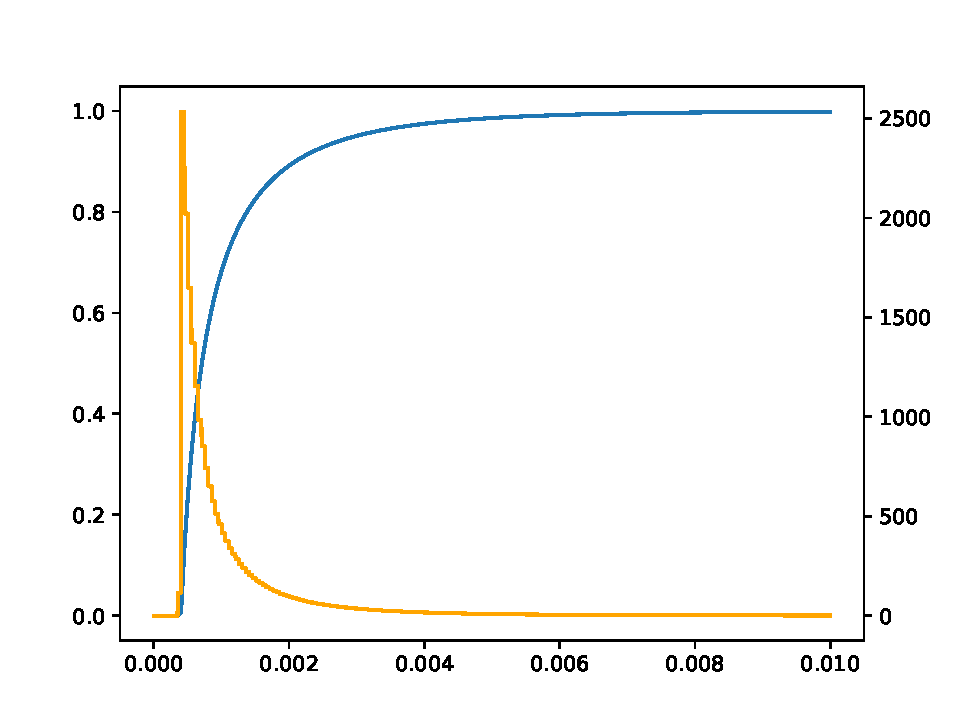
\includegraphics[width=5cm]{examples/e21_bond_slip_damage/fig_Jirasek_damage_function.pdf}}\\
\bottomrule 
\end{longtable}
}

\noindent
\begin{longtable}{L{7.5cm}L{7.5cm}}
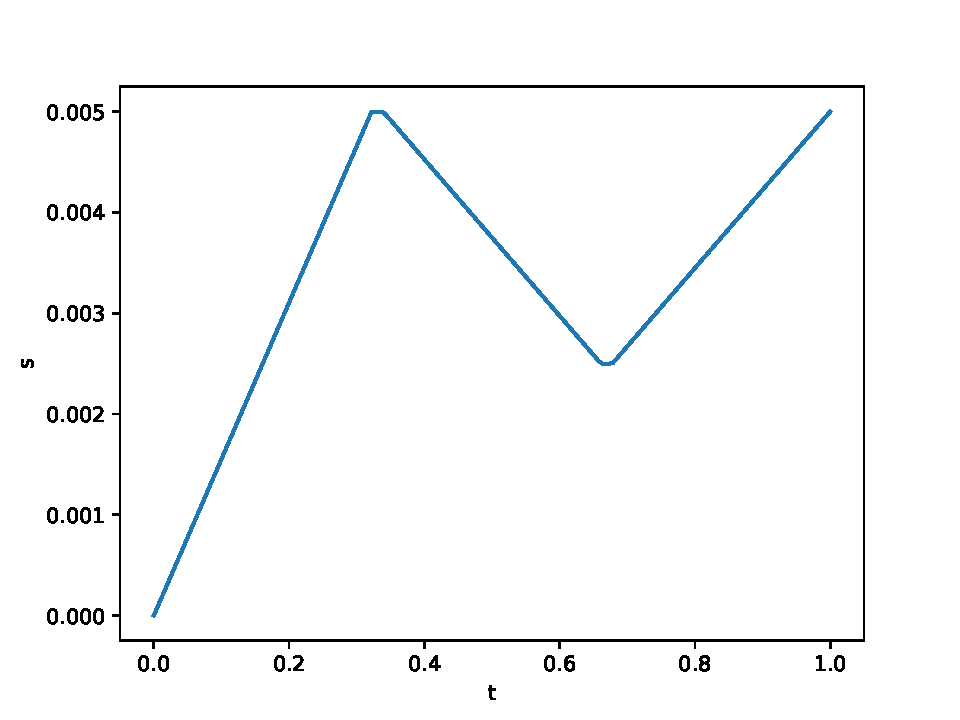
\includegraphics[width=7.5cm]{examples/e21_bond_slip_damage/fig_s-t.pdf}
 & 
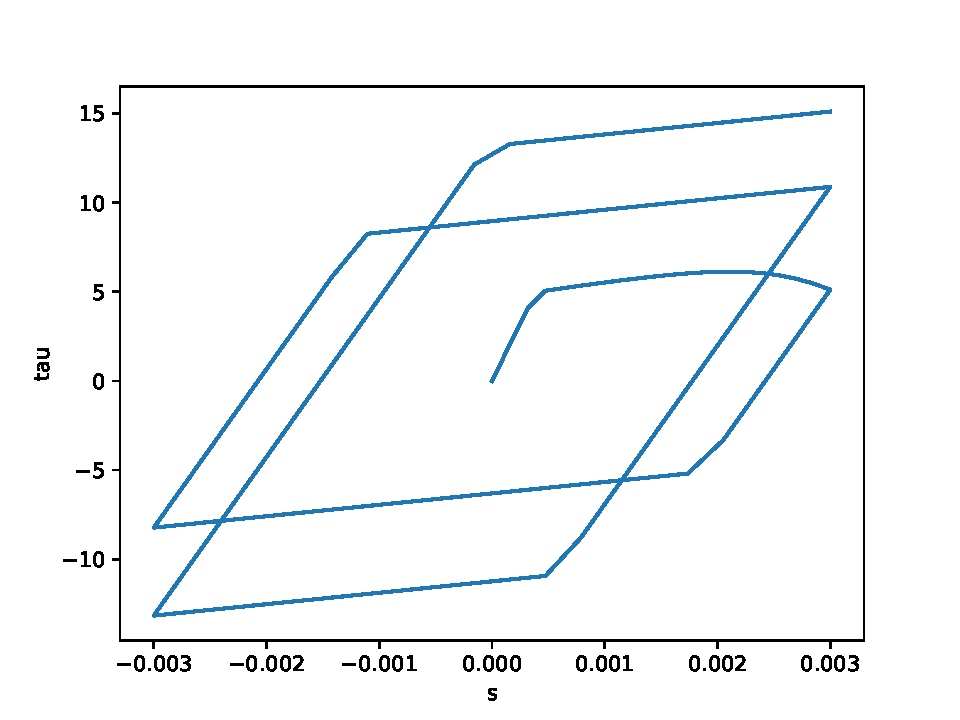
\includegraphics[width=7.5cm]{examples/e21_bond_slip_damage/fig_tau-s.pdf}
 \\\end{longtable}

\noindent
\begin{longtable}{L{7.5cm}L{7.5cm}}
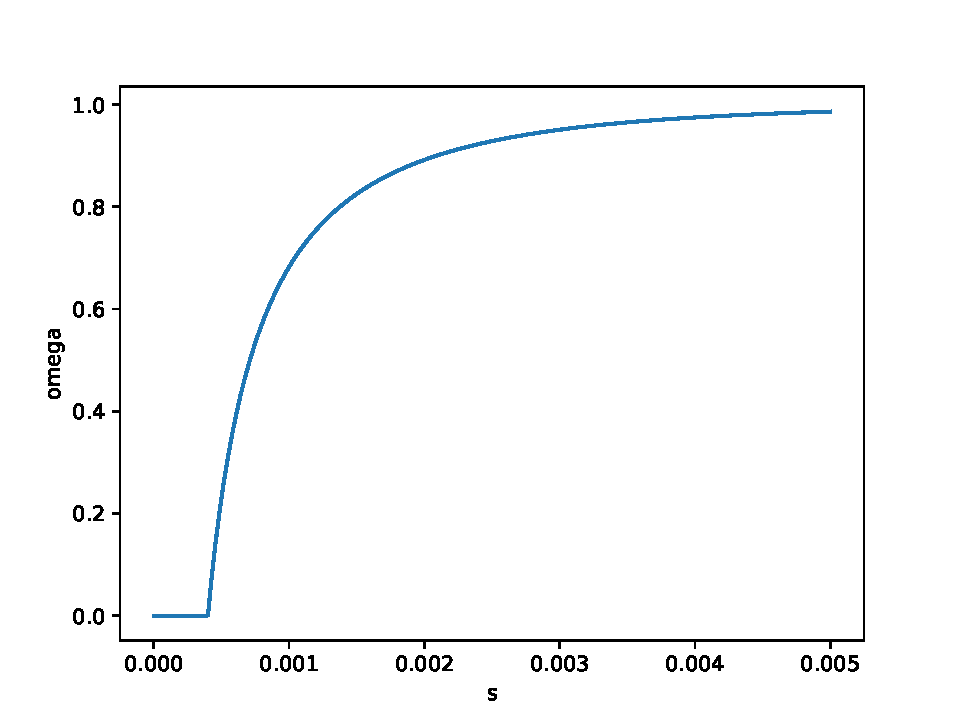
\includegraphics[width=7.5cm]{examples/e21_bond_slip_damage/fig_omega-s.pdf}
 & 
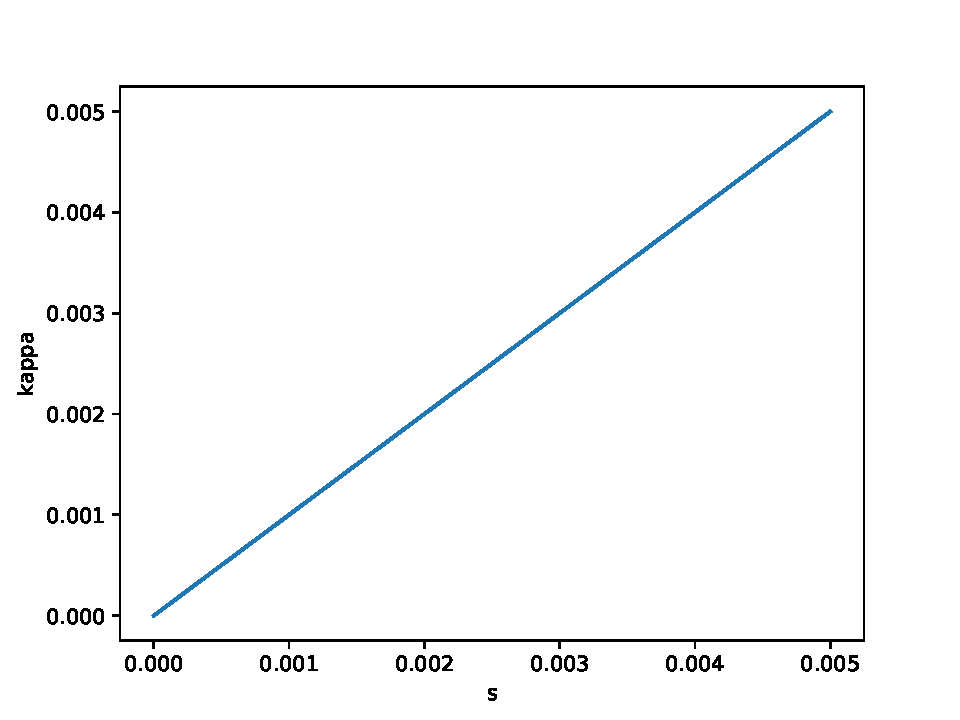
\includegraphics[width=7.5cm]{examples/e21_bond_slip_damage/fig_kappa-s.pdf}
 \\\end{longtable}
\end{center}
            \end{bmcsex}
\end{document}
    